\subsection{Minimum Vertex Cover}
The network consists of two graph convolutional layers, each consisting of an MLP with 1 layer of 100 hidden nodes.
This the output is activated through the sigmoid function, through a final graph convolution.

Firstly, the model is trained on a singular graph.
This graph is randomly generated through the \verb|networkx| package, consisting of 100 nodes.
Each edge has a $5\%$ probability of being included in the graph.
After 653 epochs, the model converges, taking approximately 1 second.
Note that the models are run in a Jupyter Notebook on an M1 mac, and are therefore not directly comparable with other methods.

The vertex cover is shown in \autoref{fig:mvc_single_graph_random}, having a size of $61$ coloured nodes, satisfying all constraints.
Additionally the number of unnecessary nodes are computed, being the number of colored nodes only connected to other colored nodes.

\begin{figure}[h]
    \centering
    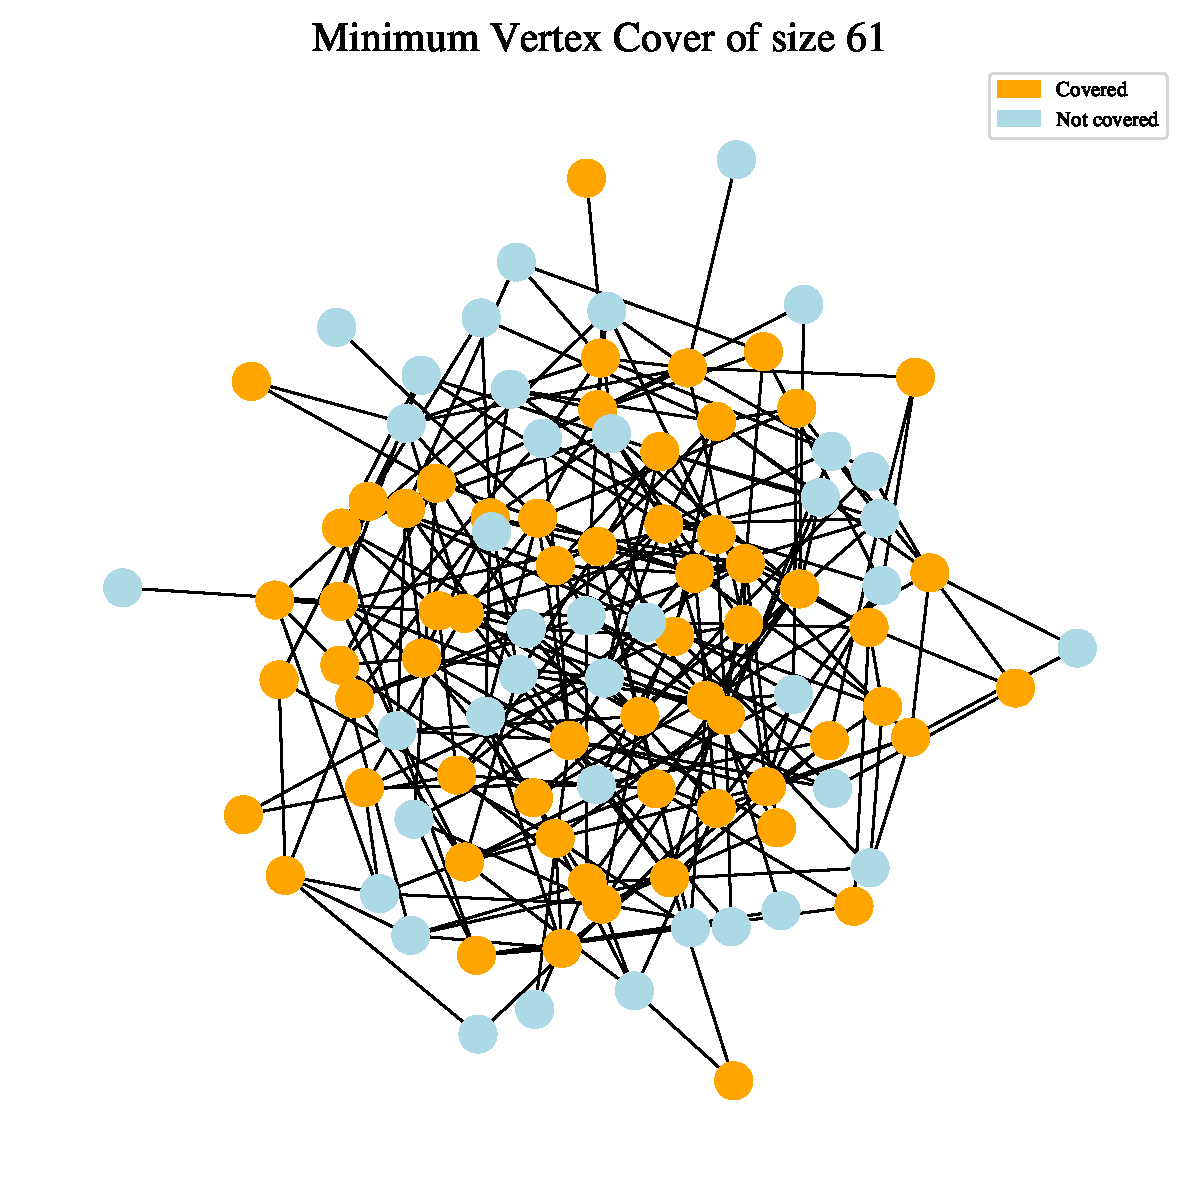
\includegraphics[width=\linewidth]{Project2TSP/_src/figures/mvc_graph_single.pdf}
    \caption{Model trained on a single random graph. Orange nodes are covered, blue are not.}
    \label{fig:mvc_single_graph_random}
\end{figure}

On such a small sample, the model is likely to be sensitive to the initial conditions of the model.
Therefore, the model is initialised on 100 random seeds, each trained on the same initial graph.
The results are presented in \autoref{table:mvc_single_seed}, showing that the model is consistently predicting a cover of around $61$.

\begin{table}[h!]
\centering
\caption{Model sensitivity to initial seed.}
\begin{tabular}{c|c|c|c}
    \toprule
    \# of & & edge & unnecessary \\
    occurrences & size & violations & colorings \\
    \colrule
    69 & 61 & 0 & 0 \\
    19 & 60 & 0 & 0 \\
    9 & 62 & 0 & 0 \\
    1 & 59 & 0 & 0 \\
    1 & 62 & 0 & 1 \\
    1 & 99 & 0 & 39 \\
    \botrule
\end{tabular}
\label{table:mvc_single_seed}
\end{table}

The predicted cover sizes are compared against the local-ratio algorithm \cite{local_ratio_approx}, guaranteeing an approximate solution which is at most twice as large as the optimal covering.
For this initial graph, the approximate cover consists of $80$ nodes, meaning our model is able to outperform it.

Finally, the model is trained on two sets of $100$ graphs, with the first being random with probability $5\%$, and the second being $3$-regular.
The models then predicts a cover for two sets of unseen graphs, being another set of random and regular graphs.

F
\begin{figure}[h]
    \centering
    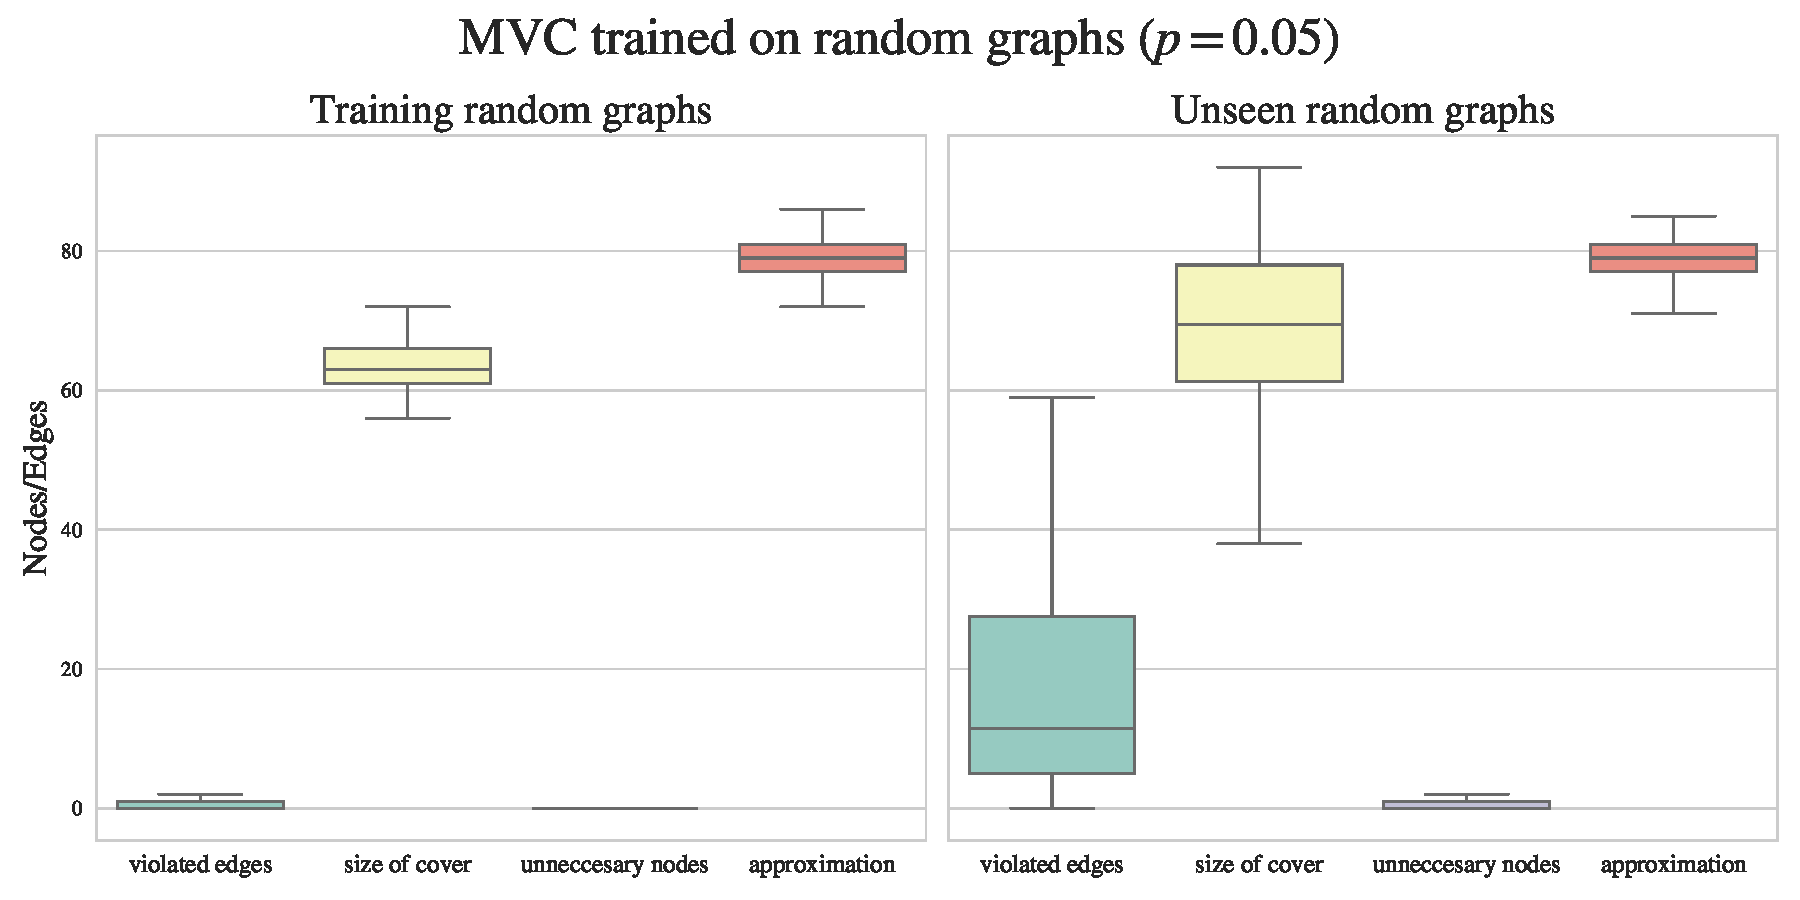
\includegraphics[width=\linewidth]{Project2TSP/_src/figures/mvc_random_boxes.pdf}
    \caption{MVC results from training on 100 random graphs, and predicting on a different set of 100 random graphs, with interquartile ranges highlighted. From left to right, the number of violated edges, sizes of the covers, uneccesary nodes and approximate solutions.}
    \label{fig:mvc_random_to_random}
\end{figure}

\begin{figure}[h]
    \centering
    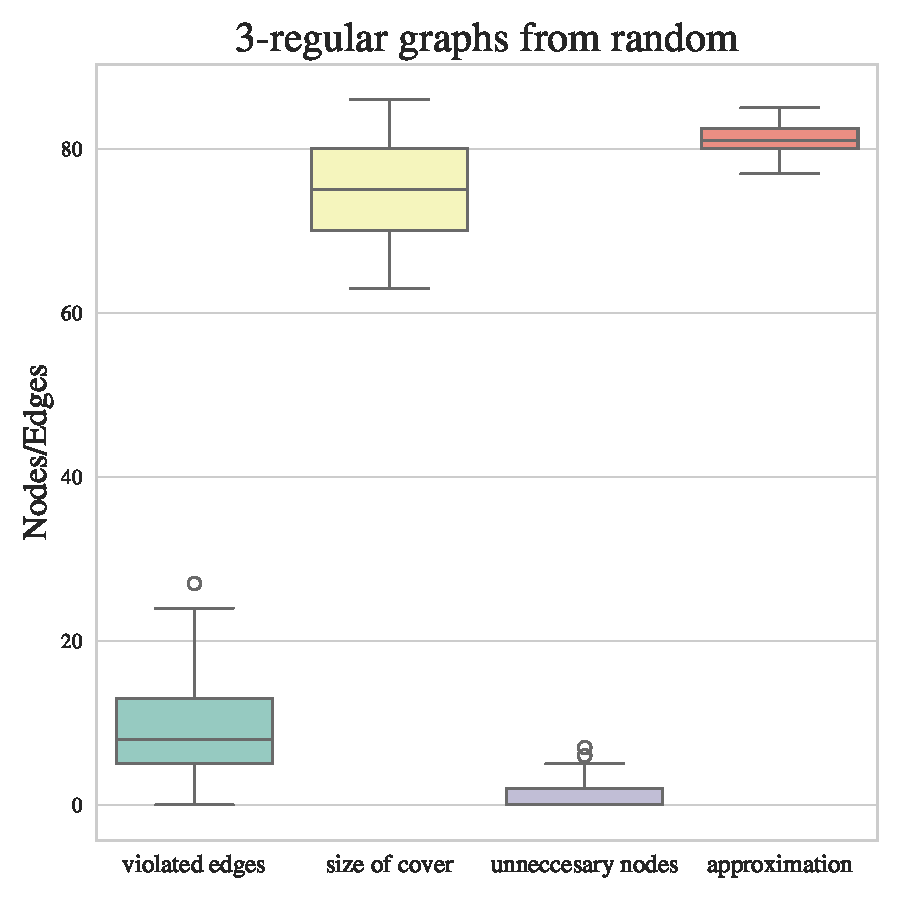
\includegraphics[width=\linewidth]{Project2TSP/_src/figures/mvc_random_to_regular.pdf}
    \caption{Caption}
    \label{fig:mvc_random_to_regular}
\end{figure}

\begin{figure}[h]
    \centering
    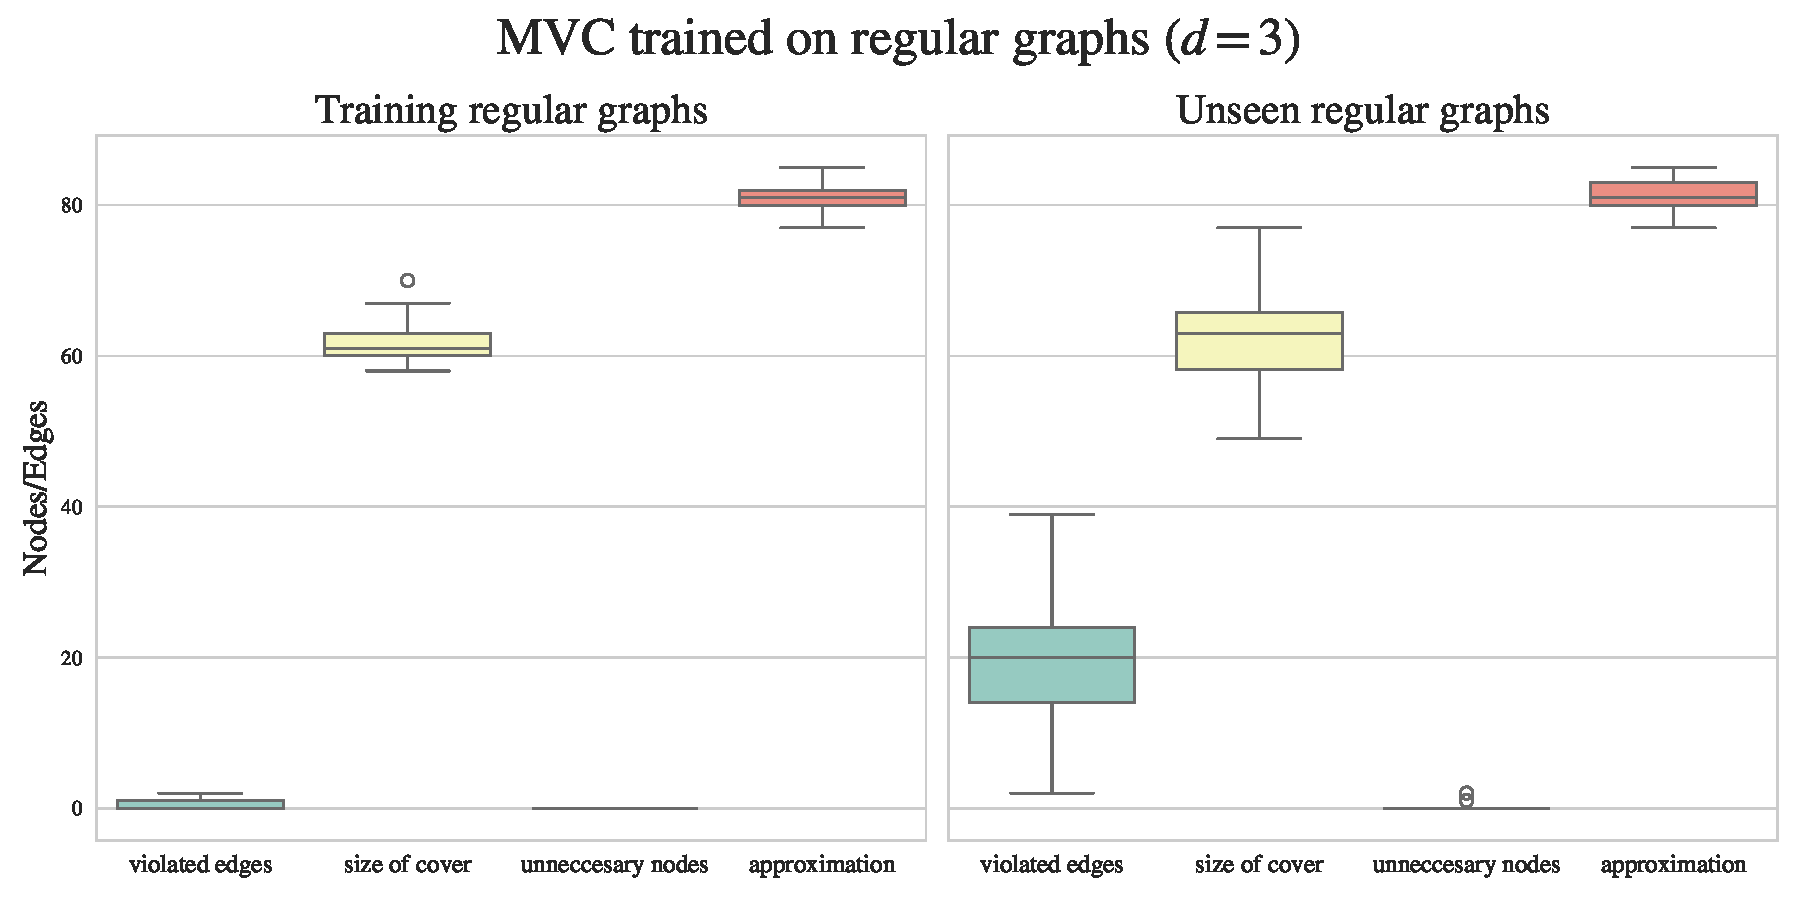
\includegraphics[width=\linewidth]{Project2TSP/_src/figures/mvc_regular_boxes.pdf}
    \caption{Caption}
    \label{fig:mvc_regular_to_regular}
\end{figure}

\begin{figure}[h]
    \centering
    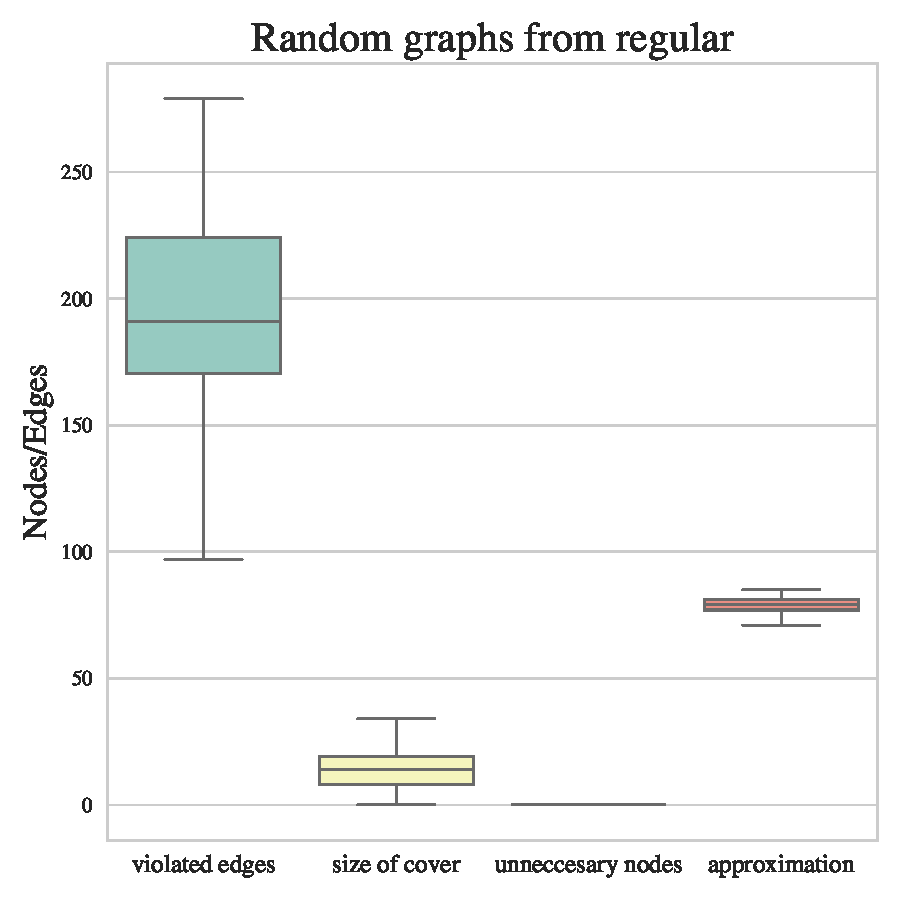
\includegraphics[width=\linewidth]{Project2TSP/_src/figures/mvc_regular_to_random.pdf}
    \caption{Caption}
    \label{fig:mvc_regular_to_random}
\end{figure}